\documentclass[12pt, a4paper, twoside]{article}
\usepackage[utf8]{inputenc}
\usepackage[cm]{fullpage}
\usepackage{fancyhdr}
\usepackage{textcomp}
\usepackage{graphicx}
\usepackage{commath}
\usepackage[portuguese]{babel}

\begin{document}

\title{Trabalho 5 da disciplina "Organização e Arquitetura de Computadores" 1 /
2018}
\author{Cristiano Silva Júnior: 13/0070629}
\date{\today}
\maketitle

\section{Introdução}

O objetivo deste trabalho é implementar o banco de registradores (BREG) do
processador MIPS desenvolvido na disciplina. O BREG deverá permitir a
recuperação de dados salvos durante a execução de um problema. Os dados somente
poderão ser salvos quando um indicador \textit{"write enable"} for verdadeiro.
Além disso, deve haver uma opção para apagar todos os dados no registrador.

\section{Metodologia}

A implementação do BREG foi feita em VHDL utilizando a ferramenta Altera Quartus
II com o auxílio do Altera ModelSim para a suíte de testes. Testes unitários
para cada operação estão contidos no arquivo "testbench.vhd" enquanto o BREG
foi implementado no arquivo "BREG.vhd".

O \textit{testbench} inclui testes unitários para o registrador 0, para o sinal
de \textit{reset}, e para escrita e leitura nos outros registradores.

\section{Resultados}

\subsection{Circuito gerado}

Por meio da implementação, pode-se gerar o circuito, que contém 3475
componentes.

O processo de leitura do banco de registradores é assíncrono, ou seja, esta
parte do circuito é reativa, enquanto a escrita só ocorre na subida do
\textit{clock} se o sinal \textit{"write enable"} estiver ativo.

\subsection{Simulação}

Utilizando o ModelSim, geramos uma simulação em forma de onda para o circuito.
No caso, mostramos a dinâmica recomendada de atribuir um valor arbitrário aos
registradores que depois são lidos em saídas diferentes

\begin{figure}
	\centering
	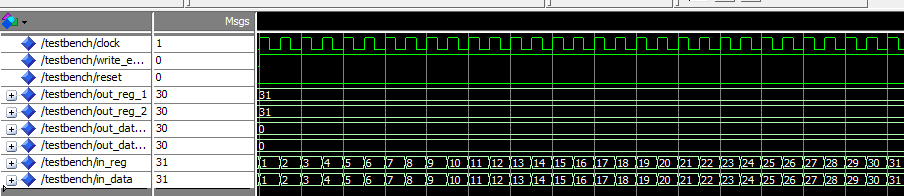
\includegraphics[width=0.8\textwidth]{docs/wave_in_reg.png}
	\caption{Escrita no banco de registradores.}
\end{figure}

A figura 1 mostra o processo de escrita no banco de registradores enquanto a
figura 2 mostra o processo de leitura do banco de registradores: dos
registradores 1 a 10, lemos pela saída 1; dos 11 a 20, pela saída 2; e da 21
em diante, das duas saídas ao mesmo tempo.

\begin{figure}
	\centering
	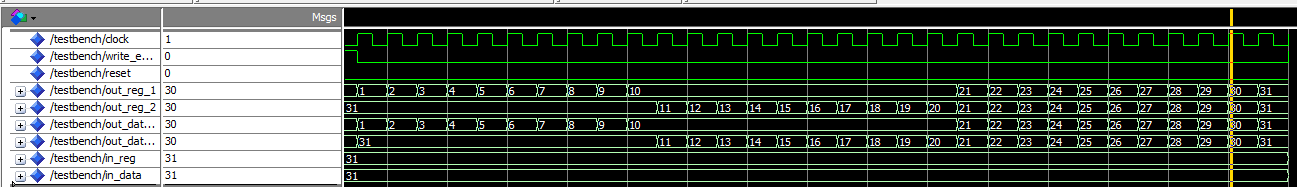
\includegraphics[width=0.8\textwidth]{docs/wave_out_reg.png}
	\caption{Leitura do banco de registradores.}
\end{figure}

\section{Conclusão}

A implementação de todao BREG proposta foi possível sem maiores problemas.

\end{document}
